% !TEX root = ../meca1321-synthesis.tex

\chapter{Transfert de chaleur}
  Un transfert de chaleur est un transfert d'énergie créé par un écart de température entre 2 points d'un milieu ou entre mileux distincs. Il existe 3 modes de transferts de chaleur: conduction, convection et rayonnement. Les deux premiers sont régis par des équations locaales (dérivées partielles) et le dernier par des équations globales (intégrales).
  \begin{itemize}
    \item La \textit{conduction} est la transmission d'énergie de proche en proche (via molécules, atomes, électrons, etc.). Elle dépend exclusivement des propriétés physiques du marériau.
    \item La \textit{convection} est la transmission d'énergie par delà une interface (\textit{e.g.} fluide-solide). Elle dépend des propriétés de conduction des deux milieux au voisinage de l'interface et de l'écoulement dans un voisinage étendu de l'interface.
    \item Le \textit{rayonnement thermique} est un rayonnement électromagnétique (spectre visible et infrarouge) pour lequel des interactions mécaniques sont possibles avec des éléments de la matière. Les solides qui absorbent les rayonnements sur une épaisseur (très) faible sont dit opaques. Les fluides, les solides restants (\textit{e.g.} verre) et certains gaz (\textit{e.g.}, $CO^2$, $H_2O$, etc.) absorbent le rayonnement partiellement et progressivement. Ils sont dits semi-transparents. Enfin, les gaz simples (\textit{e.g.} $Ar$, $O_2$, $N_2$) sont quasi-parfaitement transparents.
  \end{itemize}

  Les deux premiers transferts font appel à des lois linéaires\footnote{Dans leur formulation usuelle} tandis que la dernière ne le fait pas du tout. La loi de Stefan-Boltzman régissant le rayonnement est hautement non-linéaire, faisant intervenir $T^4$...

  \section{Transfet de chaleur dans les solides}
    \subsection{Conduction: loi de Fourier}
      Pour un matériau homogène et isotrope, le transfert de chaleur est caractérisé par la densité de flux de chaleur
      \begin{equation}
        \vb{q} = - k \grad T
      \end{equation}
      Pour rappel, $k = \hat{k}(p, T)$ est la condinuité thermique propre au matériau. Contrairement à d'autres constantes de ce type, elle varie peu dans des intervales de température limités.

      Le flux de chaleur à travers une surface $A$ avec une densité $q(\vb{n})$
      \begin{equation}
        \mathcal{Q} = \int_A q(\vb{n}) dA = \int_A \vb{q} \cdot \vb{n} dA
      \end{equation}
      L'équation de conservation de la chaleur est alors
      \begin{equation}
        \begin{aligned}
          \rho \pdv{U}{t} &= r - \div \vb{q}\\
          \rho c \pdv{T}{t} &= r +  \div (j \grad T)\\
          \recip{\alpha} \pdv{T}{t} &= \frac{r}{k} + \grad^2 T
        \end{aligned}
      \end{equation}
      La diffusivité thermique $\alpha$ représente la facilité avec laquelle le flux de chaleur transmis à un solide se transmet en relèvement de la température.

      \subsubsection{Conduction à travers une plaque, en régime permanent}
        Soit une plaque telle que l'épaisseur L est beaucoup plus petite que les autres dimensions. En négligeant les effets de bord, la recherche de la température est un problème 1-D.
        \begin{equation}
          \begin{aligned}
            \dv[2]{T}{x} &= 0 \quad \textrm{avec } T(0) = T_0 \textrm{ et } T(L) = T_L\\
            T(x) &= \frac{T_L - T_0}{L} x + T_0
          \end{aligned}
        \end{equation}
        la densité de flux de chaleur et le flux de chaleur à travers une aire latérale A de la plaque vaut alors
        \begin{equation}
          q = -k \frac{T_L - T_0}{L} \quad \mathcal{Q} = Aq = -A k \frac{T_L - T_0}{L}
        \end{equation}
        Le problème ici présenté est trop partiel. En effet, la plaque considérée est environnée à ses deux surfaces par des fluides dont on connaît les températures et itensités d'échange. En revanche, la temparature des parois est généralement inconnue et très difficile à mesurer.

        \begin{figure}[!h]
          \centering
          % !TEX root=meca1321-synthesis.tex
\tikzsetnextfilename{profilTempConv}
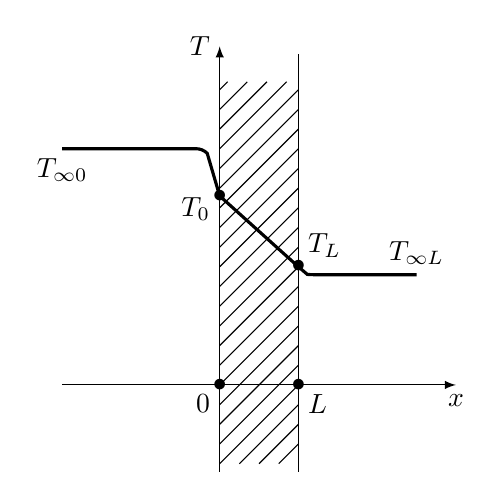
\begin{tikzpicture}
  \draw [>=latex, ->] (-2, 0) -- (3, 0) node [below] {$x$};
  \draw [>=latex, ->] (0, -1.1) -- (0, 4.3) node [left] {$T$};
  \draw (0, 0) node {$\bullet$};
  \draw (0, 0) node [below left] {$0$};
  \draw (1, 0) node {$\bullet$};
  \draw (1, 0) node [below right] {$L$};
  \draw (1, -1.1) -- (1, 4.2);
  \foreach \i in {-4, ..., 11}
  {
    \pgfmathsetmacro{\x}{(\i/4)};
    \draw (0, \x) -- ++(1, 1);
  }
  \draw (0.25, -1) -- ++(0.75, 0.75);
  \draw (0.50, -1) -- ++(0.5, 0.5);
  \draw (0.75, -1) -- ++(0.25, 0.25);
  \draw (0, 3) -- ++(0.85, 0.85);
  \draw (0, 3.25) -- ++(0.6, 0.6);
  \draw (0, 3.5) -- ++(0.35, 0.35);
  \draw (0, 3.75) -- ++(0.1, 0.1);
  \draw (0, 2.4) node {$\bullet$};
  \draw (1, 1.5) node {$\bullet$};
  \draw [line width = 0.4mm] (1, 1.5) -- (0, 2.4);
  \draw (0, 2.5) node [below left] {$T_0$};
  \draw (1, 1.5) node [above right] {$T_L$};

  \draw [line width = 0.4mm] (-2, 3) -- (-0.3, 3) arc (90:45:0.2) -- (0, 2.4);
  \draw (-2, 3) node [below] {$T_{\infty 0}$};
  \draw [line width = 0.4mm] (2.5, 1.4) -- (1.2, 1.4) arc (270:265:1) -- (1,1.5);
  \draw (2.5, 1.4) node [above] {$T_{\infty L}$};
\end{tikzpicture}

          \caption{Profil de température dans une plaque plane avec conduction (dans la plaque) et convection (en dehors) représentées}
          \label{fig:profilTempPlane}
        \end{figure}

    \subsection{Convection: Loi de Newton}
      La loi de transfert de chaleur d'une paroi de température $T_p$ à un fluide de température moyenne $T_f$ est
      \begin{equation}
        \mathcal{Q} = Ah(T_p - T_f)
      \end{equation}
      où $A$ est l'aire d'échange et $h$ le coefficient de convection. Il faut faire attention au fait que $h$ n'est pas fixe: il dépend du profil de vitesse à la paroi, des propriétés du fluide (viscosité, $k$, $\rho$, $c$, etc.). Pour ce chapitre, il est cependant considéré constant.
      \subsubsection{Plaque soumise à convection}
        Soit une plaque soumise à convection. Le profil de température au long de la plaque est continu. Les températures des parois sont $T_0$ et $T_L$ et les températures loin des parois sont $T_{\infty 0}$ et $T_{\infty L}$. Les C.L. sécrivent via le fait que le flux conduit par la plaque est le même que celui qui en sort par convection.
        \begin{equation}
          \begin{aligned}
            -k \dv{T}{x} \eval_0 &= h_0 (T_{\infty 0} - T_0) \quad \textrm{en } x = 0,\\
            -k \dv{T}{x} \eval_L &= h_L (T_{L} - T_{\infty L}) \quad \textrm{en } x = L
          \end{aligned}
        \end{equation}
        On a alors
        \begin{equation}
          T = \frac{(T_{\infty L} - T_{\infty 0})\left(\frac{x}{L} + \frac{k}{h_0 L}\right)}{1 + \frac{k}{h_0 L} + \frac{k}{h_L L}} + T_{\infty 0}
          = \frac{(T_{\infty L} - T_{\infty 0})\left(\frac{x}{L} + \recip{Bi_0}\right)}{1 + \recip{Bi_0} + \recip{Bi_L}} + T_{\infty 0}
        \end{equation}
        où $Bi$ est le nombre de Biot estimé à une paroi: $Bi_0 = \frac{h_0 L}{k}$ et $Bi_L = \frac{h_L L}{k}$. Celui-ci quantifie le rapport entre effets convectifs et conductifs.

      \subsubsection{Génération interne de chaleur dans un cylindre}
        Soit un cylindre de rayon $R$ sous génération interne de chaleur via effet Joule par un courant éléctrique dans le cylindre. Le passage d'électricité est irréversible et la transformation électricité-chaleur est une dissipation électrique. En supposant le courant uniformément réparti, la densité de puissance calorifique fournie est
        \begin{equation}
          g = \frac{I^2}{\sigma}
        \end{equation}
        où $\sigma$ est la condcuctiblité électrique $[\Omega^{-1}]$ et I est la densité de courant $[Am^{-2}]$. En régime permanent, l'équation de la chaleur est
        \begin{equation}
          \frac{g}{k} + \recip{r}\dv{r}\left(r \dv{T}{r}\right) = 0
        \end{equation}
        En supposant la dissipation de chaleur par convection, les C.L.\footnote{La deuxième traduit impossibilité de discontinuité de la densité de flux en l'absence de source le long de l'axe du cylindre} sont
        \begin{equation}
          \begin{aligned}
            -k \dv{T}{r} \eval_R &= h (T_R - T_\infty) \quad \textrm{en } r = R,\\
            -k \dv{T}{r} \eval_0 &= 0 \quad \textrm{en } r = 0
          \end{aligned}
        \end{equation}
        Le résultat est alors
        \begin{equation}
          T = \frac{gR^2}{4k}\left(1-\left(\frac{r}{R}\right)^2\right) + \frac{gR}{2h} + T_\infty
        \end{equation}

    \subsection{Notion de résistance thermique}
      Le flux $\mathcal{Q}$ peut s'écrire sous trois formes
      \begin{equation}
        \begin{aligned}
          \mathcal{Q} &= \frac{T_{\infty 0} - T_0}{\recip{Ah_0}} \quad \textrm{(convection)}\\
          \mathcal{Q} &= \frac{T_0 - T_L}{\frac{T_0}{Ak}} \quad \textrm{(conduction)}\\
          \mathcal{Q} &= \frac{T_L - T_{\infty L}}{\recip{Ah_L}} \quad \textrm{(convection)}
        \end{aligned}
      \end{equation}
      Chacune de ces expression est analogue à la loi d'Ohm $I = \frac{\Delta U}{R}$ où on pourrait distinguer deux types de résistances thermiques: conductive ($\frac{L}{Ak}$) et convective ($\recip{Ah}$). Un écart de température est ainsi un écart de potentiel thermique et le nombre de Biot le rapport entre résistivité conductivité et conductive. L'analogie peut être étendue au cas tridimensionnel en comparant la loi de Fourier à la forme vectorielle de la loi d'Ohm
      \begin{multicols}{2}
        \begin{equation}
          \vb{q} = - k  \grad T \nonumber
        \end{equation}

        \begin{equation}
          \vb{j} = - \sigma \grad U
        \end{equation}
      \end{multicols}
      où j est la densité de courant, $\sigma$ la conductance unitaire ($[\si{\Omega^{-1} m^{-2}}]$). On peut par ailleurs aussi établir que
      \begin{equation}
        \begin{aligned}
          \mathcal{Q} &= \frac{T_{\infty 0} - T_0}{\recip{Ah_0}} = \frac{T_{0} - T_L}{\frac{L}{Ak}} = \frac{T_L - T_{\infty L}}{\recip{Ah_L}}\\
          &= \frac{T_{\infty 0} - T_{\infty L}}{\recip{Ah_0} + \frac{L}{Ak} + \recip{Ah_L}}
        \end{aligned}
      \end{equation}

      \begin{figure}[!h]
        \centering
        % !TEX root = ../meca1321-synthesis.tex
\tikzsetnextfilename{profilTempRes}
\begin{tikzpicture}
  \draw [>=latex, ->] (-2, 0) -- (3, 0) node [below] {$x$};
  \draw [>=latex, ->] (0, -1.1) -- (0, 4.3) node [left] {$T$};
  \draw (0, 0) node {$\bullet$};
  \draw (0, 0) node [below left] {$0$};
  \draw (1, 0) node {$\bullet$};
  \draw (1, 0) node [below right] {$L$};
  \draw (1, -1.1) -- (1, 4.2);
  \foreach \i in {-4, ..., 11}
  {
    \pgfmathsetmacro{\x}{(\i/4)};
    \draw (0, \x) -- ++(1, 1);
  }
  \draw (0.25, -1) -- ++(0.75, 0.75);
  \draw (0.50, -1) -- ++(0.5, 0.5);
  \draw (0.75, -1) -- ++(0.25, 0.25);
  \draw (0, 3) -- ++(0.85, 0.85);
  \draw (0, 3.25) -- ++(0.6, 0.6);
  \draw (0, 3.5) -- ++(0.35, 0.35);
  \draw (0, 3.75) -- ++(0.1, 0.1);
  \draw (0, 2.4) node {$\bullet$};
  \draw (1, 1.5) node {$\bullet$};
  \draw [line width = 0.4mm] (1, 1.5) -- (0, 2.4);
  \draw (0, 2.5) node [below left] {$T_0$};
  \draw (1, 1.5) node [above right] {$T_L$};

  \draw [line width = 0.4mm] (-2, 3) -- (-0.3, 3) arc (90:45:0.2) -- (0, 2.4);
  \draw (-2, 3) node [below] {$T_{\infty 0}$};
  \draw [line width = 0.4mm] (2.5, 1.4) -- (1.2, 1.4) arc (270:265:1) -- (1,1.5);
  \draw (2.5, 1.4) node [above] {$T_{\infty L}$};

  \ctikzset{bipoles/resistor/width=0.4}
  \ctikzset{bipoles/resistor/height=0.16}
  \draw (0,-2) to[R] (1,-2);
  \draw (0,-2) node {$\bullet$};
  \draw (1,-2) node {$\bullet$};
  \draw (0,-2) to[R] (-1.5,-2);
  \draw (1,-2) to[R] (2.5,-2);
  \draw (-1.5,-2) node {$\bullet$};
  \draw (2.5, -2) node {$\bullet$};
  \draw (-1.7,-2) -- (-1.5,-2);
  \draw (-1.5,-2) node [above] {$T_{\infty 0}$};
  \draw (0,-2) node [above] {$T_{0}$};
  \draw (1,-2) node [above] {$T_{L}$};
  \draw (2.5,-2) node [above] {$T_{\infty L}$};
  \draw (2.5,-2) -- ++(0.2,0);
  \draw (-0.75,-2.5) node {$\recip{Ah_0}$};
  \draw (0.5, -2.5) node {$\frac{L}{Ak}$};
  \draw (1.75, -2.5) node {$\recip{Ah_L}$};
\end{tikzpicture}

        \caption{Circuit électrique équivalent au transfert de chaleur à travers une plaque}
        \label{fig:profilTempRes}
      \end{figure}

      Il peut être utile de définir un paramètre unique pour le transfet de chaleur. U, le coefficient global de transfert de chaleur $[\si{W \cdot m^{-2} \cdot K}]$est alors défini par
      \begin{equation}
        \mathcal{Q} = AU(T_{\infty 0} - T_{\infty L})
      \end{equation}
      avec, pour plusieurs parois
      \begin{equation}
        \recip{AU} = R_{tot} = \recip{Ah_0} + \sum_i \frac{L_i}{Ak_i} + \recip{Ah_L}
      \end{equation}

      \subsubsection{Conduction dans un tube}
        En appliquant le même raisonnement sur un tube, l'équation de Laplace s'écrit
        \begin{equation}
          \begin{aligned}
            \recip{r}\dv{r}\left(r\dv{T}{r}\right) &= 0
            T &= a log(r) + b
          \end{aligned}
        \end{equation}
        On définit les températures intérieure $T(r_i)= T_i$ et extérieure $T(r_e) = T_e$ et on obtient la solution
        \begin{equation}
          T = \frac{(T_e - T_i) \log(r)}{\log\left(\frac{r_e}{r_i}\right)} - \frac{(T_e - T_i) \log(r_e)}{\log\left(\frac{r_e}{r_i}\right)} - T_e
        \end{equation}
        La densité de flux chaleur et le flux à travers une longueur L valent
        \begin{multicols}{2}
          \begin{equation}
            q = -k \frac{T_e - T_i}{r\log\left(\frac{r_e}{r_i}\right)} \nonumber
          \end{equation}

          \begin{equation}
            \mathcal{Q} = 2\pi Lrq = -2\pi L k \frac{T_e - T_i}{\log\left(\frac{r_e}{r_i}\right)}
          \end{equation}
        \end{multicols}

        % Si on veut introduire les effets conductifs, on a
        % \begin{itemize}
        %   \item en $r = r_i$, $\quad -k \dv{T}{r}\eval_{r_i} = h_i (T_{\infty i} - T_i)$
        %   \item en $r = r_e$, $\quad -k \dv{T}{r}\eval_{r_e} = h_e (T_e - T_{\infty e})$
        % \end{itemize}

  \section{Transfert thermique établi}
    On considère des "transferts thermiques établis" (défini plus loin) avec écoulement établi en conduite circulaire. Le profil de vitesse est donc $u(r) = 2 u_m \left(1 - \left(\frac{r}{R}\right)\right)$. On néglige la condition de chaleur dans la direction axiale car elle est faible par rapprot à la radiale ou nulle $\left(\pdv[2]{T}{x} \ll \recip{r}\pdv{r}\left(r\pdv{T}{r}\right)\right)$. L'équation de l'énergie est alors
    \begin{equation}
      \rho c u \pdv{T}{x} = k \recip{r}\pdv{r} \left(r\pdv{T}{r}\right) + \mu \left(\dv{u}{r}\right)^2 \quad \textrm{avec } \dv{u}{r} = -4\frac{u_mr}{R^2}
    \end{equation}

    La température moyenne\footnote{En anglais, \textit{cup mixing temperature}} $T_m$, représentative du flux de chaleur au sein de la conduite, est
    \begin{equation}
      cT_m = \frac{\int_A c T \rho u dA}{\int_A \rho u dA}
    \end{equation}
    Dans le cas d'un écoulement incompressible avec $c$ constant, on a
    \begin{equation}
      T_m = \frac{\int_A T u dA}{\int_A u dA} = \frac{\int_A T u dA}{u_m A}
    \end{equation}
    Le flux énergétique global au sein de la conduite est alors égal à $c T_m \rho u_m A$.

    Le \textit{nombre de Nusselt} est le coefficient adimensionnel de transfert de chaleur défini comme
    \begin{equation}
      Nu = \frac{q_w D}{k (T_w - T_m)} = \frac{h D}{k}
    \end{equation}
    où $T_w$ est la température à la paroi, $q_w$ la densité de flux de chaleur à la paroi $q_w = k \frac{dT}{dr}\eval_r=R$ et $D$ le diamètre de la conduite.

    Il est aussi très utile de considérer le bilan d'énergie perdue/acquise par l'écoulement sur une longueur $dx$. On intègre d'abord le terme de dissipation visqueuse au travers de la section
    \begin{equation}
      \int_A \left(\dv{u}{r}\right)^2 dA = 16 \mu u_m^2 2\pi \int_0^R \left(\frac{r}{R}\right)^2 \frac{r}{R} \frac{dr}{R} = 32 \pi\mu u_m^2 \int_0^1 \eta^3 d\eta = 8 \pi \mu u_m^2
    \end{equation}
    \begin{figure}[!h]
      \centering
      % !TEX root=meca1321-synthesis.tex
\tikzsetnextfilename{transThermCond}
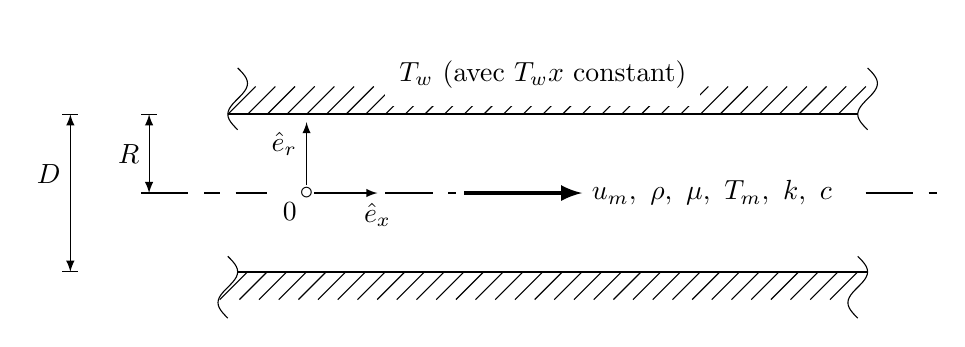
\begin{tikzpicture}
  % Tracé des parois
  \draw [thick] (-4,1) -- (4,1);
  \draw [domain=-pi:pi] plot ({sin(deg(\x))/8-3.875},{((\x+pi/2)/8+1});
  \draw [domain=-pi:pi] plot ({sin(deg(\x))/8+4.125},{((\x+pi/2)/8+1});
  \draw [thick] (-3.875,-1) -- (4.125,-1);
  \draw [domain=-pi:pi] plot ({sin(deg(\x))/8-4},{((\x-pi/2)/8-1});
  \draw [domain=-pi:pi] plot ({sin(deg(\x))/8+4},{((\x-pi/2)/8-1});
  \foreach \i in {0,...,31}
  {
    \pgfmathsetmacro{\x}{(- 4 + \i/4)};
    \draw (\x,1) -- ++(45:0.5);
    \draw (\x+1/4,-1) -- ++(-135:0.5);
  }
  %Repères et autres flèches
  \draw [dash pattern= on 0.6cm off 0.2cm on 0.2cm off 0.2cm] (-5.1,0) -- (-3.5,0);
  \draw [>=latex,<->] (-6,-1) -- (-6,1);
  \draw (-5.1,1) -- ++(0.2,0);
  \draw (-5,0.5) node [left] {$R$};
  \draw [>=latex,<->] (-5,0) -- (-5,1);
  \draw (-6.1,1) -- ++(0.2,0);
  \draw (-6.1,-1) -- ++(0.2,0);
  \draw (-6,0) node [above left] {$D$};
  \draw (-3,0) node {$\circ$};
  \draw (-3,0) node [below left] {$0$};
  \draw [>=latex,->] (-3,0.1) -- (-3,0.9);
  \draw [>=latex,->] (-2.9,0) -- (-2.1,0);
  \draw (-3.0,0.9) node [below left] {$\hat{\vb{e}}_r$};
  \draw (-2.1,0) node [below] {$\hat{\vb{e}}_x$};
  \draw [dash pattern= on 0.6cm off 0.2cm on 0.2cm off 0.2cm] (-2,0) -- (-1.1,0);
  \draw [ultra thick,>=latex,->] (-1,0) -- (0.5,0);
  \draw (0.5,0) node [right] {$u_m,~\rho,~\mu,~T_m,~k,~c$};
  \draw [dash pattern= on 0.6cm off 0.2cm on 0.2cm off 0.2cm] (4.1,0) -- (5,0);
  \fill [white] (-2, 1.1) rectangle (2, 2.1);
  \draw (0, 1.5) node {$T_w$ (avec $\dv{T_w}{x}$ constant)};

\end{tikzpicture}

      \caption{Transfert thermique établi en conduite circulaire}
      \label{fig:transthermCond}
    \end{figure}

    On obtient alors le bilan suivant
    \begin{equation}
      \begin{aligned}
        (q_w 2\pi R + 8 \pi \mu u_m^2) dx &= (\rho u_m \pi R^2)cdT_m\\
        \rho u_m c \dv{T_m}{dx} &= \frac{4}{D} q_w + 32 \mu \left(\frac{u_m}{D}\right)^2
      \end{aligned}
    \end{equation}

    Lorsque $T_w > T_m$, $q_w$ est positif et de la chaleur est transférée de la paroi vers l'écoulement ($T_m$ augmente avec x) et vice-versa. Dans les deux cas, le nombre de Nusselt est positif. Si $q_w$ est constant, alors $\dv{T_m}{x}$ l'est aussi.

    Un transfert thermique est établii si le profil normalisé adimensionnel de différence de température $\frac{T - T_w}{T_m - T_w}$ ne dépend pas de $x$.
    \begin{equation}
      \begin{aligned}
        0 &= \pdv{x} \left(\frac{T-T_w}{T_m - T_w}\right)\\
        &= \recip{T_m - T_w} \left(\pdv{T}{x} - \dv{T_w}{x}\right) - \frac{T-T_w}{(T_m - T_w)^2} \left(\dv{T_m}{x} - \dv{T_w}{x}\right)
      \end{aligned}
    \end{equation}

    Comme $\frac{T - T_w}{T_m - T_w}$ ne dépend que de $r$, c'est le cas aussi pour la dérivée. En $R$, celle-ci vaut $-Nu/D$: Nusselt est indépendant de $x$ pour le transfert thermique établi.

    \begin{figure}[!h]
      \centering
      % !TEX root = ../meca1321-synthesis.tex

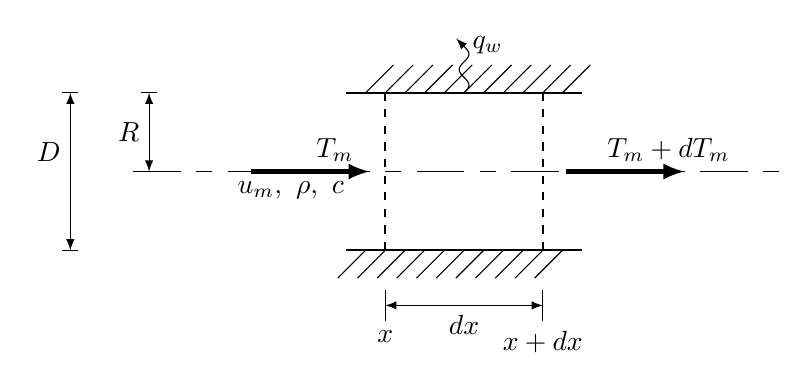
\begin{tikzpicture}
  % Tracé des parois
  \draw [thick] (-1.5,1) -- (1.5,1);
  \draw [thick] (-1.5,-1) -- (1.5,-1);
  \foreach \i in {0,...,10}
  {
    \pgfmathsetmacro{\x}{(- 1.5 + \i/4)};
    \draw (\x+1/4,1) -- ++(45:0.5);
    \draw (\x+1/4,-1) -- ++(-135:0.5);
  }
  %Repères et autres flèches
  \draw [>=latex,<->] (-5,-1) -- (-5,1);
  \draw (-4.1,1) -- ++(0.2,0);
  \draw (-4,0.5) node [left] {$R$};
  \draw [>=latex,<->] (-4,0) -- (-4,1);
  \draw (-5.1,1) -- ++(0.2,0);
  \draw (-5.1,-1) -- ++(0.2,0);
  \draw (-5,0) node [above left] {$D$};
  \draw [dash pattern= on 0.6cm off 0.2cm on 0.2cm off 0.2cm] (-4.2,0) -- (4,0);
  \draw [ultra thick,>=latex,->] (-2.7,0) -- ++(1.5,0);
  \draw [thick, dashed] (-1, -1) -- (-1, 1);
  \draw [thick, dashed] (1, -1) -- (1, 1);
  \draw [ultra thick,>=latex,->] (1.3, 0) -- ++(1.5,0);
  \draw (3.5, 0) node [above left] {$T_m + dT_m$};
  \draw (-2, 0) node [above right] {$T_m$};
  \draw (-3, 0) node [below right] {$u_m,~\rho,~c$};
  \draw (-1, -1.5) -- ++(0, -0.4) node [below] {$x$};
  \draw (1, -1.5) -- ++(0, -0.4) node [below] {$x+dx$};
  \draw [>=latex,<->] (-1, -1.7) -- ++(2, 0);
  \draw (0, -1.7) node [below] {$dx$};
  \draw [domain=0:3*pi] plot ({sin(deg(\x))/16}, {\x/16+1}) [>=latex, ->] -- ++(-0.1,0.1);
  \draw (0.3, 1.6) node {$q_w$};
\end{tikzpicture}

      \caption{Bilan d'énergie thermique perdue (acquise) par l'écoulemeent établi sur un élément différentiel de longueur $dx$}
      \label{bilanEnerg}
    \end{figure}

    \subsection{Transfert thermique établi avec température de paroi constante}
      À température de paroi constante, on a que $\dv{T_w}{x} = 0$ et donc
      \begin{equation}
        \pdv{T}{x} = \frac{T-T_w}{T_m - T_w} \dv{T_m}{x}
      \end{equation}

      \subsubsection{Cas à température moyenne d'écoulement constante}
        Si la température moyenne d'écoulement est constante, on a
        \begin{equation}
          \pdv{T}{x} = 0
        \end{equation}
        La conduction de chaleur dans la direction axiale s'annule ici parfaitement. L'équation de l'énergie est alors
        \begin{align}
          0 &= k \recip{r} \dv{r}\left(r\dv{T}{r}\right) + \mu \left(\dv{u}{r}\right)^2\\
          k \recip{r} \dv{r}\left(r\dv{r}(T-T_w)\right) &= - 16\mu \frac{u_m^2}{R^2} \left(\frac{r}{R}\right)^2 \\ \intertext{Par intégration}
          T-T_w &= \frac{\mu u_m^2}{k} \left(1-\left(\frac{r}{R}\right)^4\right)
        \end{align}
        La température maximale est la rempérature au centre $T_c$
        \begin{equation}
          T_c - T_w = \mu \frac{\mu u_m^2}{k}
        \end{equation}
        Le transfert de chaleur à la paroi est
        \begin{equation}
          q_w = k \dv{T}{r}\eval_{r=R} = -4\mu \frac{u_m^2}{R} = -4k \frac{T_c - T_w}{R}
        \end{equation}
        On obtient aussi (avec $dA = rd\theta dr$ et $\eta = r/R$)
        \begin{equation}
          T_m - T_w = \recip{u_m \pi R^2} \frac{\mu}{k} u_m^2 2 u_m 2\pi R^2 \int_0^1(1-\eta^4)(1-\eta^2) \eta d\eta = \frac{5}{6} \frac{\mu}{k} u_m^2
        \end{equation}
        Et donc
        \begin{multicols}{3}
          \begin{equation}
              \frac{T-T_w}{T_m - T_w} = \frac{6}{5} \left(1 - \left(\frac{r}{R}\right)^4\right) \nonumber
          \end{equation}

          \begin{equation}
            q_w = -\frac{24}{5}k\frac{T_m - T_w}{R} \nonumber
          \end{equation}

          \begin{equation}
            Nu = \frac{48}{5} = 9.60
          \end{equation}
        \end{multicols}

      \subsubsection{Cas à température d'écoulement moyenne d'écoulement variable}
        Dans ce cas, l'équation de l'énergie
        \begin{equation}
          \rho \frac{T-T_w}{T_m - T_w}\dv{T_m}{x} 2 u_m \left(1 - \left(\frac{r}{R}\right)^2\right) = k \dv{r}\left(r \dv{r}(T-T_w)\right)
        \end{equation}
        En répétant les étapes précédentes, on peut obtenir un nombe de Nusselt $Nu \simeq 3.66$. Ce nombre est constant selon $x$, malgré le fait que $q_w$ ne le soit pas.

    \subsection{Transfert thermique établi avec température de paroi et température moyenne linéaires et de même pente}
      \begin{equation}
        \pdv{T}{x} = \dv{T_w}{x} = \dv{T_m}{x} = cste \quad \Longrightarrow \quad \pdv[2]{T}{x} = 0
      \end{equation}
      Il n'y a pas de conduction de chaleur dans la direction axiale. L'équation de bilan d'énergie implique un $q_w$ constant en $x$.
      L'équation d'énergie devient alors
      \begin{equation}
        \rho c \dv{T}{x} 2 u_m \left(1 - \left(\frac{r}{R}\right)^2\right) = k \recip{r} \dv{r}\left(r \dv{r}(T - T_w)\right) + 16 \mu \frac{u_m^2}{R^2} \left(\frac{r}{R}\right)^2
      \end{equation}
      Par intégration
      \begin{equation}
        T-T_w = \frac{\mu u_m^2}{k} \left(1-\left(\frac{r}{R}\right)^4\right) - \frac{\rho c}{8k} \dv{T_w}{x} u_m R^2 \left(3-4\left(\frac{r}{R}\right)^2 + \left(\frac{r}{R}\right)^4\right)
      \end{equation}
      Il s'agit de la solution exacte du problème. Définissons le paramètre adimensionnel $\beta$
      \begin{equation}
        \beta = \frac{\frac{\rho c}{k}\dv{T_w}{x} u_m R^2}{\frac{\mu}{k}{u_m^2}} = \rho c \dv{T_w}{x}\frac{R^2}{\mu u_m}
      \end{equation}
      On a alors
      \begin{equation}
        \begin{aligned}
          T-T_w &= \frac{\mu u_m^2}{k} \left( \left(1-\left(\frac{r}{R}\right)^4\right) - \frac{\beta}{8} \left(3-4\left(\frac{r}{R}\right)^2 + \left(\frac{r}{R}\right)^4\right)\right)\\
          T_m -T_w &= \frac{\mu u_m^2}{k} \left(\frac{5}{6} - \frac{11}{48}\beta\right)\\
          \frac{q_w D}{k} &= - \frac{\mu}{k} u_m^2 (8-\beta)\\
          \frac{T-T_w}{T_m - T_w} &= \frac{\left(1-\left(\frac{r}{R}\right)^4\right) - \frac{\beta}{8} \left(3-4\left(\frac{r}{R}\right)^2 + \left(\frac{r}{R}\right)^4\right)}{\frac{5}{6} - \frac{11}{48}\beta}\\
          Nu &= \frac{q_w}{k(T_w - T_m)} = \frac{8-\beta}{\frac{5}{6} - \frac{11}{48}\beta}
        \end{aligned}
      \end{equation}

      On constate que $\beta=0$ correspond au cas à température de paroi constante tandis que $\beta=8$ correspond à un cas adiabatique. $\beta=\frac{40}{11}$ correspond à un cas $Nu \rightarrow \infty$. On note aussi le cas $\beta \rightarrow \pm \infty$. On a alors
      \begin{equation}
        \begin{aligned}
          T-T_w &= -\frac{\rho c}{8k} \dv{T_w}{x} u_m R^2 \left(3-4\left(\frac{r}{R}\right)^2 + \left(\frac{r}{R}\right)^4\right)\\
          T_m -T_w &= - \frac{11}{48} \frac{\rho c}{k} \dv{T_w}{x} u_m R^2 \\
          q_w &= -\recip{2} \rho c \dv{T_w}{x} u_m R\\
          \frac{T-T_w}{T_m - T_w} &= \frac{6}{11}\left(3-4\left(\frac{r}{R}\right)^2 + \left(\frac{r}{R}\right)^4\right)\\
          Nu &= \frac{q_w}{k(T_w - T_m)} = \frac{48}{11}
        \end{aligned}
      \end{equation}
      On a aussi quel que soit $\beta$
      \begin{equation}
        \frac{T-T_w}{T_m-T_w} = \frac{9}{8} \quad \textrm{ en } \frac{r}{R} = \recip{2}
      \end{equation}

      \begin{figure}[!h]
        \centering
        % !TEX root = meca1321-synthesis.tex
\tikzsetnextfilename{profilDiffTempNeg}
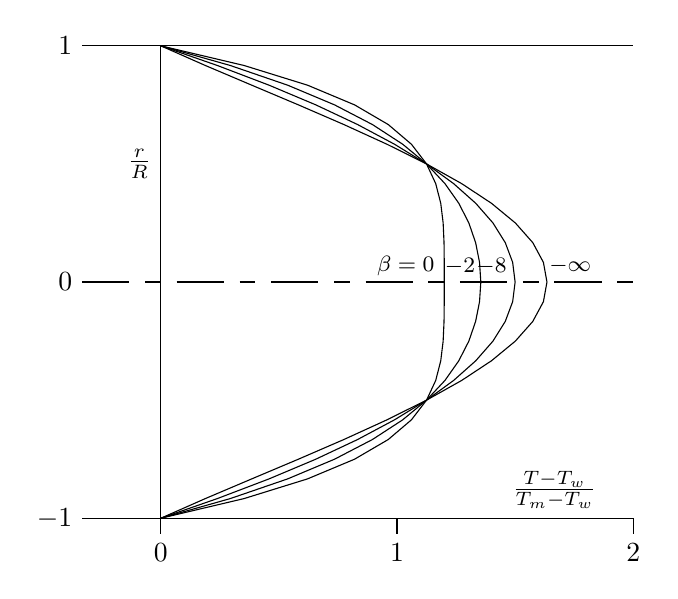
\begin{tikzpicture}
  \draw (0,-3) -- ++(0,6);
  \draw (-1, -3) node [left] {$-1$}-- ++(7,0);
  \draw (-1, 3) node [left] {$1$}-- ++(7,0);
  \draw [dash pattern= on 0.6cm off 0.2cm on 0.2cm off 0.2cm] (-1,0) node [left] {$0$} -- ++(7,0);
  \foreach \i in {0,1,2}
  {
    \draw (\i*3, -3) -- ++(0, -0.2) node [below] {$\i$};
  }
  \foreach \i in {0, -2, -8, -1000}
  {
    \draw [domain=-1:1] plot ({3*((1-(\x)^(4)) - 0.125*\i*(3-4*(\x)^(2) + (\x)^(4)))/((5/6)-(11/48)*\i)},{3*\x});
  }
  \draw (3.6,0.2) node [left] {\footnotesize$\beta=0$};
  \draw (3.8,0.2) node {\footnotesize$-2$};
  \draw (4.2,0.2) node {\footnotesize$-8$};
  \draw (5.2,0.2) node {\footnotesize$-\infty$};
  \draw (0, 1.5) node [left] {$\frac{r}{R}$};
  \draw (5, -3) node [above] {$\frac{T - T_w}{T_m - T_w}$};
\end{tikzpicture}

        \caption{Profils adimensonnels de différence de température pour le transfert thermique établi en conduite circulaire: cas avec $\beta \geq 0$}
        \label{fig:profilDiffTempNeg}
      \end{figure}

      \begin{figure}[!h]
        \centering
        % !TEX root = ../meca1321-synthesis.tex
\tikzsetnextfilename{profilDiffTempPos}
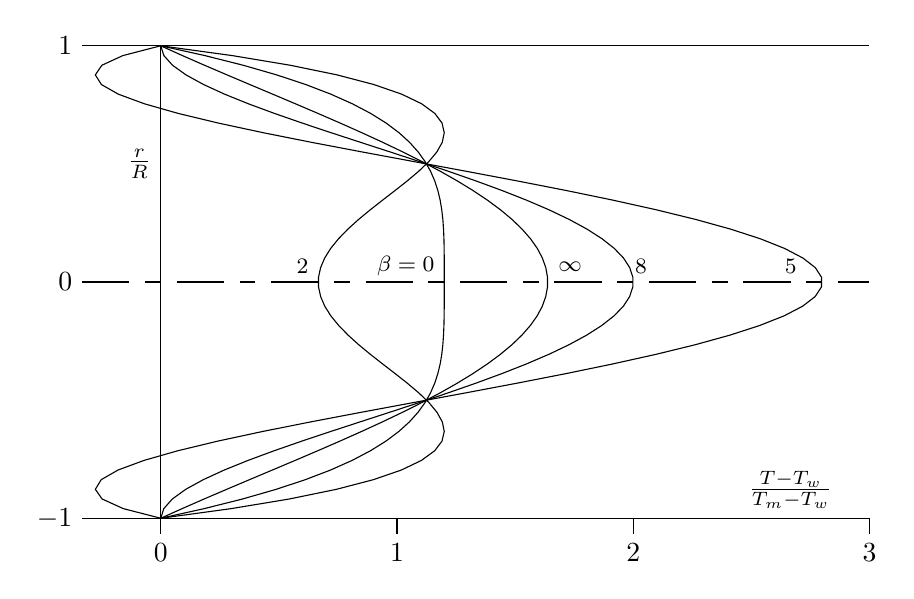
\begin{tikzpicture}
  \draw (0,-3) -- ++(0,6);
  \draw (-1, -3) node [left] {$-1$}-- ++(10,0);
  \draw (-1, 3) node [left] {$1$}-- ++(10,0);
  \draw [dash pattern= on 0.6cm off 0.2cm on 0.2cm off 0.2cm] (-1,0) node [left] {$0$} -- ++(10,0);
  \foreach \i in {0,...,3}
  {
    \draw (\i*3, -3) -- ++(0, -0.2) node [below] {$\i$};
  }
  \foreach \i in {0, 2, 5, 8, 1000}
  {
    \draw [domain=-1:1, samples=50] plot ({3*((1-(\x)^(4)) - 0.125*\i*(3-4*(\x)^(2) + (\x)^(4)))/((5/6)-(11/48)*\i)},{3*\x});
  }
  \draw (3.6,0.2) node [left] {\footnotesize$\beta=0$};
  \draw (2,0.2) [left] node {\footnotesize$2$};
  \draw (5.2,0.2) node {\footnotesize$\infty$};
  \draw (6.1,0.2) node {\footnotesize$8$};
  \draw (8,0.2) node {\footnotesize$5$};
  \draw (0, 1.5) node [left] {$\frac{r}{R}$};
  \draw (8, -3) node [above] {$\frac{T - T_w}{T_m - T_w}$};
\end{tikzpicture}

        \caption{Profils adimensonnels de différence de température pour le transfert thermique établi en conduite circulaire: cas avec $\beta \leq 0$}
        \label{fig:profilDiffTempPos}
      \end{figure}

      \begin{figure}[!h]
        \centering
        % !TEX root = ../meca1321-synthesis.tex
\tikzsetnextfilename{nusseltVar}
\begin{tikzpicture}[scale=0.8]
  \draw [>=latex,->] (0, -4) -- ++(0, 8);
  \draw [>=latex,->] (-5.5,0) -- ++(11, 0);
  \foreach \i in {-3,-2,...,3}
  {
    \draw (-0.1, \i) -- ++(0.2, 0);
  }
  \foreach \i in {-4, -3,..., 4}
  {
    \draw (\i, -0.1) -- ++(0, 0.2);
  }
  \draw [domain=-27.5:2.4, samples=100] plot({\x/5},{(8-\x)/(((5/6) - (11/48)*\x)*5)});
  \draw [domain= 4.4:27.5, samples=100] plot({\x/5},{(8-\x)/(((5/6) - (11/48)*\x)*5)});
  \draw (5.5, 1) node [left] {$Nu$};
  \draw [domain=-27.5:27.5,samples=100, dotted] plot ({\x/5},{((5/6) - (11/48)*\x)/5)});
  \draw [domain=-12.5:27.5,samples=100, dashed] plot ({\x/5},{(8-\x)/5});
  \draw (5.5, 0) node [below left] {$\beta$};
  \draw (5.5, -3) node {$\frac{q_w}{\frac{\mu u_m^2}{D}}$};
  \draw (-5, 2) node {$\frac{T_m -T_w}{\frac{\mu u_m^2}{k}}$};
  \draw (0, 1) node [left] {$5$};
  \draw (1, 0) node [below] {$5$};
  \draw (0, 0) node [below left] {$0$};
\end{tikzpicture}

        \caption{Variation du nombre de Nusselt en fonction de $\beta$ pour le transfert thermique établi en conduite circulaire}
        \label{fig:nusseltVar}
      \end{figure}

    \subsection{Entrée thermique: le problème de Grätz}
      Considérons le problème du développement d'un profil de température dans un écoulement établi suite à un changement brusque de température. Pour $x<0$, $T=T_0$ et, pour $x>0$, $T=T_w\neq T_0$.

      \begin{figure}[!h]
        \centering
        % !TEX root = ../meca1321-synthesis.tex

\tikzsetnextfilename{gratz}
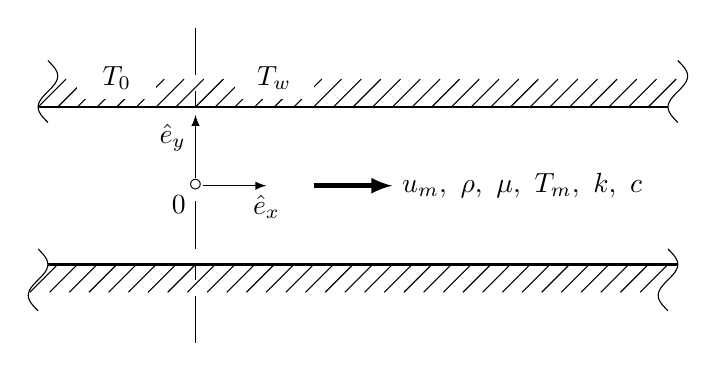
\begin{tikzpicture}
  % Tracé des parois
  \draw [thick] (-4,1) -- (4,1);
  \draw [domain=-pi:pi] plot ({sin(deg(\x))/8-3.875},{((\x+pi/2)/8+1});
  \draw [domain=-pi:pi] plot ({sin(deg(\x))/8+4.125},{((\x+pi/2)/8+1});
  \draw [thick] (-3.875,-1) -- (4.125,-1);
  \draw [domain=-pi:pi] plot ({sin(deg(\x))/8-4},{((\x-pi/2)/8-1});
  \draw [domain=-pi:pi] plot ({sin(deg(\x))/8+4},{((\x-pi/2)/8-1});
  \foreach \i in {0,...,31}
  {
    \pgfmathsetmacro{\x}{(- 4 + \i/4)};
    \draw (\x,1) -- ++(45:0.5);
    \draw (\x+1/4,-1) -- ++(-135:0.5);
  }
  %Repères et autres flèches
  \draw (-2,0) node {$\circ$} node [below left] {$0$};
  \draw [>=latex,->] (-2,0.1) -- (-2,0.9);
  \draw [>=latex,->] (-1.9,0) -- (-1.1,0);
  \draw (-2.0,0.9) node [below left] {$\hat{\vb{e}}_y$};
  \draw (-1.1,0) node [below] {$\hat{\vb{e}}_x$};
  \draw [ultra thick,>=latex,->] (-0.5,0) -- (0.5,0);
  \draw (0.5,0) node [right] {$u_m,~\rho,~\mu,~T_m,~k,~c$};
  \draw [dash pattern= on 0.6cm off 0.2cm on 0.2cm off 0.2cm] (-2,-2) -- (-2,-0.2);
  \draw [dash pattern= on 0.6cm off 0.2cm on 0.2cm off 0.2cm] (-2,0.2) -- (-2,2);
  \fill (-0.5, 1.1) [white] rectangle (-1.5, 2);
  \draw (-1, 1.1) node [above] {$T_w$};
  \fill (-2.5, 1.1) [white] rectangle (-3.5, 2);
  \draw (-3, 1.1) node [above] {$T_0$};
\end{tikzpicture}

        \caption{Entrée thermique avec écoulement de Poiseuille en conduite circulaire}
      \end{figure}

      En considérant le cas avec dissipatiton visqueuse négligeable, l'équation d'énergie est
      \begin{equation}
        \rho c u \pdv{T}{x} = k \recip{r} \pdv{r}\left(r\pdv{T}{r}\right)
      \end{equation}
      Avec la diffusivité thermique $\alpha = \frac{k}{\rho c} = \frac{\nu}{Pr}$
      \begin{equation}
        u \pdv{T}{x} = \alpha \recip{r} \pdv{r}\left(r\pdv{T}{r}\right)
      \end{equation}

      Dans le cas d'un écoulement de Poiseuille, $u = 2u_m \left(1 - \left(\frac{r}{R}\right)^2\right)$
      \begin{equation}
        2u_m \left(1 - \left(\frac{r}{R}\right)^2\right) \pdv{T}{x} = \alpha \recip{r} \pdv{r} \left(r\pdv{T}{r}\right)
      \end{equation}
      Les variables adimensionnel sont
      \begin{equation}
        T^\ast = \frac{T-T_w}{T_0 - T_w}, \quad \eta = \frac{r}{R}, \quad \zeta = \recip{Re_D Pr} \frac{x}{D} = \recip{Pe_D} \frac{x}{D}
      \end{equation}
      et $Pe_D = Re_D Pr$, le nombre de Peclet. L'équation devient
      \begin{equation}
        (1-\eta^2) \pdv{T^\ast}{\zeta} = \frac{2}{\eta} \pdv{\eta} \left(\eta \pdv{T^\ast}{\eta}\right), \quad T^\ast (\eta, 0) = 1, \quad T^\ast (1, \zeta) = 0
      \end{equation}
      L'équation est à variable séparable, de la forme
      \begin{equation}
        T^\ast (\eta, \zeta) = f(\eta)g(\zeta)
      \end{equation}
      Après résolution\footnote{Voir page 79}, on obtient
      \begin{equation}
        \begin{aligned}
          T^\ast (\eta, \zeta) &= 2 \sum_{n=1}^\infty \frac{J_0 (\lambda_n \eta)}{\lambda_n J_1(\lambda_n)} e^{-4\lambda_n^2 \zeta}\\
          \pdv{T^\ast}{\eta} &= -2 \sum_{n=1}^\infty \frac{J_1(\lambda_n \eta)}{J_1(\lambda_n)} e^{-4\lambda_n^2 \zeta}
        \end{aligned}
      \end{equation}

      Le transfeert de chaleur à la paroi
      \begin{equation}
        q_w(\zeta) = k \pdv{T}{r}\eval_{r=R} = \frac{k}{R}(T_0 - T_w) \pdv{T^\ast}{\eta} \eval_{\eta = 1} = -\frac{k}{R} (T_0 - T_w) 2 \sum_{n=1}^\infty e^{-4 \lambda_n^2 \zeta}
      \end{equation}
      La température moyenne de référence utilisée pour définir le nombre de Nusselt est
      \begin{equation}
        \frac{T_m - T_w}{T_0 - T_w} = T_m^\ast(\zeta) = \frac{\int T^\ast u dA}{u_m A} = \frac{\int T^\ast dA}{A} = 2 \int_0^1 T^\ast(\eta, \zeta) \eta d\eta = 4 \sum_{n=1}^{\infty} \recip{\lambda_n^2}e^{-4 \lambda_n^2 \zeta}
      \end{equation}
      où on utilis $u=u_m$ dans un problème simplifié avec écoulement bouchon. Le nombre de Nusselt
      \begin{equation}
        Nu(\zeta) = \frac{q_w D}{k (T_w - T_m)} = \frac{\sum_{n=1}{\infty} e^{-4 \lambda_n^2 \zeta}}{\sum_{n=1}^\infty \recip{\lambda_n^2} e^{-4 \lambda_n^2 \zeta}}
      \end{equation}

      La longueur caractéristique est donnée par le terme exponentiel le plus petit: $\zeta_c \approx \recip{4 \lambda_1^2}$. Le transfert de chaleur asymptotique est obtenu
      \begin{equation}
        Nu(\zeta > \zeta_c) \approx \lambda_1^2 = 5.78
      \end{equation}

    \subsection{Nombre de Nusselt moyen}
      Le flux de chaleur moyen sur une distance $x$ est
      \begin{equation}
        q_{w,m} (x) = \recip{x} \int_0^x q_w(x') dx'
      \end{equation}
      On peut établir le bilan d'énergie global
      \begin{equation}
        2\pi R x q_{w, m}(x) = \pi R^2 \rho u_m c (T_m(x) - T_m(0))
      \end{equation}
      qui permet d'établir l'énergie gagnée ou dissipée sur une distance $x$
      \begin{equation}
          x q(w, m) = - \frac{D}{4} \rho u_m c (T_m(x) - T_m(0)) = \recip{4}Re_D Pr k (T_m(x) - T_m(0))
      \end{equation}
      L'éuation différentielle de bilan peut aussi s'exprimer en terme du nombre de Nusselt
      \begin{equation}
        \begin{aligned}
          d(x q_{w,m}(x)) = q_w(x) dx &= \frac{D}{4} \rho u_m c dT_m\\
          Nu(x)dx = \frac{q_w(x) D}{k (T_w - T_m)} dx &= \frac{D^2}{4} \frac{\rho u_m c}{k} \frac{dT_m}{T_w - T_m}\\
          &= \frac{D}{4} Re_D Pr \frac{dT_m}{T_w - T_m}
        \end{aligned}
      \end{equation}

      Par conséquent, par intégration,
      \begin{equation}
        x Nu(x) = \frac{D}{4} Re_D Pr \log\frac{T_w - T_m(0)}{T_w - T_m(x)}
      \end{equation}
      Le nombre de Nusselt est alors le transfert de chaleur moyen normalisé
      \begin{equation}
        Nu_m(x) = \frac{q_{w,m}(x) D}{k \Delta T_m} \quad \textrm{avec } \Delta T_m = \frac{T_m(x) - T_m(0)}{\log \frac{T_w - T_m(0)}{T_w - T_m(x)}}
      \end{equation}
      $\Delta T_m$ est ici la référence pour la différence globale de température, une "moyenne logarithmique".
